\chapter{Timing Characteristics of the Program}\label{ConnectingBreakoutBoard} 
\textbf{Name: Group 630}\\
\textbf{Date: 11/05 - 2016}

\subsubsection{Purpose}
Check the proper behavior of the program running on the microcontroller to ensure proper operation of the control system.

\subsubsection{Setup}
\begin{figure}[H]
  \centering
  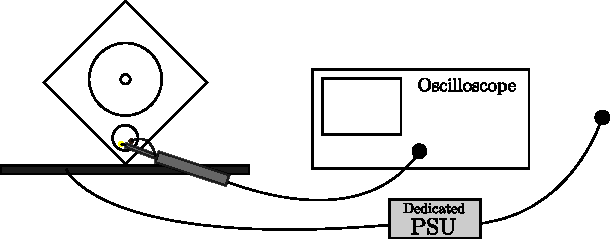
\includegraphics[scale=1]{figures/LabSetupRangeTest.pdf}
  \caption{Setup diagram}
  \label{LabSetupRangeTest}
\end{figure}
\fxnote{Modify picture to probe on the BBB}
To measure timing characteristics, it is necessary to connect to external pins of the BeagleBone Black and raise and lower the pin around the interesting program area in the source code. Here, the section of interest is the whole function \lstinline{runController()} which performs the sensor readings and runs the controller computations.\\
It should be made sure that the current sent to the motor controller is null, so that the wheel stands still while doing the measurement.

\subsubsection{List of Equipment}
\begin{table}[H]
  \begin{tabular}{|l|l|p{4.3cm}|}
    \hline%------------------------------------------------------------------------------------------------------------
    \textbf{Instrument}                                   &  \textbf{AAU-no.} &  \textbf{Type}            \\
    \hline%------------------------------------------------------------------------------------------------------------
    Oscilloscope                                          &  3386             &  Agilent 54621A           \\
    \hline%------------------------------------------------------------------------------------------------------------
    Dedicated Power Supply of Cubli \small{(24 V - 3 A)}  &                   &  XP Power, AEB70US24      \\
    \hline%------------------------------------------------------------------------------------------------------------
    Probe                                                 &                   &  1:1                      \\
    \hline%------------------------------------------------------------------------------------------------------------
  \end{tabular}
\end{table}

\subsubsection{Procedure}
\begin{enumerate}
  \item Make the setup with connections as seen on \figref{LabSetupRangeTest}, with ground on pin 2 and signal on pin 26 of the P8 header on the BeagleBone Black.
  \item Launch the appropriate program over a USB SSH connection.
  \item Set the oscilloscope on rolling and calibrate it so that a few periods of the pulse signals can be clearly seen on the display.
  \item Stop the acquisition and save the data to a floppy-disk as a CSV file. Gather the CSV log file generated by the program, from the BeagleBone Black.
\end{enumerate}

\subsubsection{Results}
